\documentclass[12pt,twoside]{article}
\usepackage[utf8]{inputenc}
\usepackage{jmlda}
\setcounter{page}{17}
\newcommand{\hdir}{.}

\newcommand{\x}{\mathbf{x}}
\newtheorem{Th}{Утверждение}

\title
    [Метрическое обучение]
    {Метрическое обучение и снижение размерности пространства в задачах кластеризации}
\author
    [Р.\,В.~Исаченко]
    {Р.\,В.~Исаченко, А.\,М.~Катруца}
\email
    {isa-ro@yandex.ru, amkatrutsa@yandex.ru}
\organization
    {Московский физико-технический институт, г. Долгопрудный, Институтский пер., 9}
\abstract
    {
    Работа посвящена использованию методов метрического обучения в задачах кластеризации.
    Применение метрического обучения позволяет модифицировать расстояния между объектами,
    сближая объекты из одного кластера и отдаляя объекты из разных кластеров.
    В данной работе расстояние измеряется при помощи метрики Махаланобиса.
    Процедура метрического обучения состоит в определении оптимальной матрицы ковариаций множества объектов.
    Кластеризация осуществляется алгоритмом $k$-средних и алгоритмом адаптивного метрического обучения, понижающим размерность признакового пространства.
    Для сравнения этих методов произведен вычислительный эксперимент на
синтетических  и реальных данных, сделан вывод об эффективности рассматриваемых методов.

\bigskip
\noindent
\textbf{Ключевые слова}: \emph {кластеризация; $k$-средних; алгоритм
адаптивного метрического обучения; $EM$-алгоритм}}

\thanks{Проект поддержан грантом РФФИ \No \ 16-37-00485.}

\titleEng
    {Metric learning and dimensionality reduction in clustering}
\authorEng
    {R.\,V.~Isachenko and A.\,M.~Katrutsa}
\thanksEng{The work was supported by the Russian Foundation for Basic Research (grant No.\,16-37-00485).}
\organizationEng
    {Moscow Institute of Physics and Technology, 9 Institutskiy per., Dolgoprudny, Moscow, Russia}
\abstractEng
    {\noindent
    This paper investigates incorporation of metric learning approach in
clustering problem. Distance metric is a key issue in many machine learning
algorithms, especially in unsupervised learning where distance between objects is the only known information.
    The metric learning procedure modifies distances between objects to make objects from the same cluster closer
    and from the different clusters more distant.
    In this paper, Mahalanobis distance is used as a~distance between objects.
    The goal of the paper is to learn Mahalanobis metric by optimizing the covariance matrix of objects according to their cluster labels.
    In this case, metric learning procedure is formulated as optimization problem.
    For clustering, $k$-means were used as baseline algorithm and Adaptive Metric Learning (AML)
algorithm.
    To solve the problem, AML algorithm uses iterative EM
(expectation-maximization) procedure to find the optimum.
    To compare these algorithms, the computational experiment was
carried out in MatLab on synthetic data and real data from UCI repository and
conclusions about performance of these algorithms have been made.

\noindent
    \textbf{Keywords}: \emph{clustering; $k$-means;
adaptive distance metric learning; $EM$-algorithm}}

\receivedRus{24.02.2016}
\receivedEng{February 24, 2016}
\doi{10.21469/22233792.2.1.02}

\begin{document}
\maketitle
\section{Введение}
Методы метрического обучения~\cite{yang2006distance, bellet2013survey}
применяются при идентификации лиц~\cite{guillaumin2009you}, классификации
текстовых документов~\cite{yang2006efficient}, распознавании рукописных
цифр~\cite{globerson2005metric}.
В~данной работе решается задача метрического обучения при кластеризации объектов на заданное количество кластеров~\cite{xing2003distance}.
Требуется выявить наборы объектов, похожих между собой, причем степень сходства определяется расстоянием между объектами.
Целью метрического обуче\-ния является выбор оптимального способа измерения расстояния между объектами.

Для решения данной задачи в работе~\cite{geurts2001pattern} используются деревья принятия решений~\cite{friedl1997decision}, основанные на логических схемах.
Но проблема построения оптимального дерева является $\NP$-полной, и практическое применение данного метода основано на эвристических алгоритмах~\cite{hyafil1976constructing}.
Другой подход к кластеризации используется в статье~\cite{dy2004feature}, где предложен эффективный  способ отбора признаков, а в качестве алгоритма кластеризации выбран
EM (expectation-maximization) алгоритм.
В работе~\cite{ye2007adaptive} для кластеризации объектов применяется
метрическое обуче\-ние.
Эта работа используется в настоящем исследовании в качестве базовой.

Предлагаемый алгоритм адаптивного метрического обучения объединяет задачи
клас\-те\-ри\-за\-ции и метрического обучения в одну задачу максимизации функционала качества.
Ключевой идеей алгоритма адаптивного метрического обучения является понижение размерности пространства объектов таким образом, чтобы расстояния между кластерами были максимальны.
Для решения оптимизационной задачи используется EM-подход.
На каждой итерации алгоритм находит ортогональное преобразование, понижающее размерность признакового пространства, и кластеризует объекты в новом пространстве.

В данной работе алгоритм адаптивного метрического обучения применяется к синтетическим и реальным данным.
Цель эксперимента~--- показать работоспособность предложенного подхода и провести его сравнение с базовым алгоритмом.
В качестве базового для сравнения алгоритма выбран алгоритм $k$-средних~\cite{macqueen1967some}.
Данный алгоритм минимизирует суммарное квадратичное отклонение точек кластеров от центров этих кластеров.
Получена оценка качества работы построенного алгоритма.
Проведен сравнительный анализ результатов, полученных с помощью метрического обучения и без него.

\section{Постановка задачи метрического обучения}
Пусть $\mathbf{X} = [\x_1, \ldots, \x_N] \in \mathbb{R}^{T \times N}$~--- множество объектов.
Объект $\mathbf{x}_i = [x_i^1, \ldots, x_i^T]^\top$ задан в виде вектора в пространстве признаков.
Требуется выявить кластерную структуру данных и разбить множество объектов $\mathbf{X}$ на множество непересекающихся кластеров,
т.\,е.\ построить отображение
\[
    a: \mathbf{X} \to \{1, \dots, K\}.
\]
Обозначим $y_i = a (\x_i)$, $y_i \in \{1, \ldots, K\}$,~--- метка кластера объекта $\x_i$.
Необходимо выбрать метки кластеров $\{y_i\}_{i=1}^N$ таким образом, чтобы расстояния между кластерами были максимальными.
Центр $\boldsymbol{\mu}$ множества объектов $\mathbf{X}$ и центры кластеров $\{\boldsymbol{\mu}_k\}_{k=1}^K$ вычисляются по формулам:
\begin{equation}
    \label{mu}
    \boldsymbol{\mu} =\frac1N \sum_{i=1}^N\x_i\,; \quad
    \boldsymbol{\mu}_k =\frac{ \sum_{i=1}^N [y_i = y_k]\mathbf{x}_i } {\sum_{i=1}^N [y_i = y_k]}\,.
\end{equation}
Введем на множестве объектов $\mathbf{X}$ расстояние Махаланобиса
\begin{equation}
    \label{metric}
    \rho (\x_i, \x_j) = \sqrt{(\x_i - \x_j)^{\top} \mathbf{A}^{-1} (\x_i - \x_j)}\,,
\end{equation}
где $\mathbf{A}$~--- это матрица ковариаций множества $\mathbf{X}$
\begin{equation}
\label{covMatrix}
    \mathbf{A} = \frac 1N \sum_{i=1}^N(\x_i - \boldsymbol{\mu})(\x_i - \boldsymbol{\mu})^{\top}.
\end{equation}
\begin{Def}
Функционалом качества кластеризации $Q$ назовем межкластерное расстояние:
\[
    Q (\{\boldsymbol{\mu}_k\}_{k=1}^K)= \sum_{k=1}^K N_k \rho^2(\boldsymbol{\mu}_k, \boldsymbol{\mu})\,,
\]
где $N_k = \sum_{i=1}^N [y_i = y_k]$~--- число объектов в кластере $k$.
\end{Def}

Поставим задачу кластеризации как задачу максимизации функционала
\begin{equation}
\label{Qmax}
    Q \bigl(\{\boldsymbol{\mu}_k\}_{k=1}^K\bigr) \to \max_{\boldsymbol{\mu}_k \in \mathbb{R}^T}.
\end{equation}
Для улучшения качества решения этой задачи предлагается применить метод метрического обучения к ковариационной матрице $\mathbf{A}$.
Найдем такую матрицу $\mathbf{A}$, для которой функционал качества принимает максимальное значение:
\begin{equation}
\label{Amax}
    \mathbf{A}^* = \mathop{\arg \max}_{\mathbf{A} \in \mathbb{R}^{T \times T}} Q \bigl(\{\boldsymbol{\mu}_k^*\}_{k=1}^K \bigr)\,,
\end{equation}
где $\{\boldsymbol{\mu}_k^*\}_{k=1}^K$~--- решение задачи кластеризации~(\ref{Qmax}).

\section{Алгоритм адаптивного метрического обучения}
Для решения поставленных оптимизационных задач~(\ref{Qmax}), (\ref{Amax}) используется алгоритм адаптивного метрического обучения.
Предлагается понизить размерность пространства объектов $\mathbf{X}$ с помощью линейного ортогонального преобразования $\mathbf{G} \in \mathbb{R}^{T \times L}$, $\mathbf{G}^{\top} \mathbf{G} = \mathbf{I}$, где новая размерность $L < T$
\[
    \mathbf{X} \ni \x_i  \mapsto \hat{\x}_i = \mathbf{G}^\top \x_i \in \mathbb{R}^L, \quad i = 1, \ldots, N.
\]
Центр $\hat{\boldsymbol{\mu}}$ множества объектов $\{\hat{\x}_i\}_{i=1}^N$ вычисляется по формуле~(\ref{mu}). Расстояния между объектами вычисляются по формуле~(\ref{metric}), где в качестве матрицы $\hat{\mathbf{A}}$ используется матрица ковариаций~(\ref{covMatrix}) множества объектов $\{\hat{\x}_i\}_{i=1}^N$

\[
    \hat{\mathbf{A}} =
    \frac 1N \sum_{i=1}^N (\hat{\x}_i - \hat{\boldsymbol{\mu}})(\hat{\x}_i - \hat{\boldsymbol{\mu}})^\top =
    \frac 1N \sum_{i=1}^N \mathbf{G}^{\top}(\x_i - \boldsymbol{\mu})(\x_i - \boldsymbol{\mu})^\top \mathbf{G} =  \mathbf{G}^{\top} \mathbf{A} \mathbf{G}.
\]
\begin{Def}
Индикаторной матрицей назовем матрицу $\mathbf{F} = \{\delta_{ik}\} \in \mathbb{R}^{N \times K}$, где
\[
\delta_{ik} =
\begin{cases}
1, & \text{если $a(\x_i) = y_k$;} \\
0, & \text{если $a(\x_i) \neq y_k$.}
\end{cases}
\]
\end{Def}
\begin{Def}
Взвешенной индикаторной матрицей назовем матрицу
$\mathbf{L} = \mathbf{F} (\mathbf{F}^{\top} \mathbf{F})^{-1/2} = \{l_{ik}\} \in \mathbb{R}^{N \times K}$, элементы которой равны:
\[
     l_{ik} =
     \begin{cases}
    \displaystyle    \frac 1{\sqrt{N_k}}, & \text{если $a(\x_i) = y_k$;} \\
        0, & \text{если $a(\x_i) \neq y_k$.}
     \end{cases}
\]
\end{Def}
\begin{Th}
C использованием данных обозначений задача кластеризации~(\ref{Qmax})
и~задача метрического обучения~(\ref{Amax}) сводятся к общей задаче максимизации функционала качества~\cite{ding2005equivalence}
\begin{equation}
\label{GLmax}
    Q = \frac 1N \Tr (\mathbf{L}^{\top} \mathbf{X}^{\top} \mathbf{G} \hat{\mathbf{A}}^{-1} \mathbf{G}^{\top} \mathbf{X L}) = \frac 1N \Tr (\mathbf{L}^{\top} \mathbf{X}^{\top} \mathbf{G}
    (\mathbf{G}^{\top} \mathbf{A G})^{-1} \mathbf{G}^{\top} \mathbf{X L}) \to \max_{\mathbf{G}, \mathbf{L}}.
\end{equation}
\end{Th}
\section{Решение задачи метрического обучения}
Для решения задачи~(\ref{GLmax}) алгоритм адаптивного метрического обучения использует \mbox{EM-под}\-ход.
На каждом шаге итеративно вычисляются локальные оптимальные значения матриц $\mathbf{G}$ и $\mathbf{L}$.
На $E$-шаге необходимо найти матрицу $\mathbf{L}$, которая является решением оптимизационной задачи~(\ref{GLmax}) при фиксированной матрице $\mathbf{G}$.
В качестве начального приближения получим взвешенную индикаторную матрицу $\mathbf{L}$ с помощью алгоритма кластеризации $k$-средних с евклидовой метрикой.
На $M$-шаге производится нахождение оптимального значения матрицы $\mathbf{G}$ при фиксированной матрице $\mathbf{L}$.
Алгоритм завершается при стабилизации функционала $Q$ на последовательности итераций.

\paragraph{Алгоритм $k$-средних}
В данной работе базовым алгоритмом для сравнения является алгоритм $k$-средних.
Первым шагом алгоритм выбирает из множества $\mathbf{X}$ случайным образом $K$ объектов $\{\boldsymbol{\mu}_k\}_{k=1}^K$~--- начальные центры кластеров.
Для каждого объекта $\x_i$ вычисляется расстояние~(\ref{metric}) до каждого центра кластера $\boldsymbol{\mu}_k$ с единичной матрицей трансформаций.
Объект~$\x_i$ относится к кластеру, расстояние до которого оказалось наименьшим.
Далее производится вычисление новых центров кластеров по формуле~(\ref{mu}).
Алгоритм завершается, если значения центров кластеров прекращают меняться.

\paragraph{Оптимизация матрицы G с фиксированной матрицей L}
Для любых двух квадратных матриц $\mathbf{A}$ и $\mathbf{B}$ справедливо $\text{trace}(\mathbf{AB}) = \text{trace}(\mathbf{BA})$.
Данное свойство позволяет переформулировать задачу~(\ref{GLmax}) следующим образом:
\[
    Q = \frac 1N \Tr (\mathbf{L}^{\top} \mathbf{X}^{\top} \mathbf{G} (\mathbf{G}^{\top} \mathbf{A G})^{-1} \mathbf{G}^{\top} \mathbf{X L}) = \frac 1N \Tr \bigl((\mathbf{G}^{\top} \mathbf{A G})^{-1} \mathbf{G}^{\top} \mathbf{X L L}^{\top} \mathbf{X}^{\top} \mathbf{G}\bigr).
\]
\begin{Th}
     Обозначим $\mathbf{B} = \mathbf{X L L}^{\top} \mathbf{X}^{\top}$.
     Обозначим через $\mathbf{G} = [\mathbf{v}_1, \ldots, \mathbf{v}_K]$ матрицу, состоящую из $K$ собственных векторов матрицы $\mathbf{A}^{-1}\mathbf{B}$, отвечающих наибольшим собственным значениям.
     Тогда решением~(\ref{GLmax}) является ортогональная матрица, полученная $QR$-раз\-ло\-же\-ни\-ем матрицы $\mathbf{G}$.
\end{Th}

Функционал качества $Q$ зависит только от матрицы $\mathbf{G}$. Обозначим
\[
    s(\mathbf{G}) = \Tr \bigl((\mathbf{G}^{\top} \mathbf{A G})^{-1} \mathbf{G}^{\top} \mathbf{B G}\bigr).
\]
На данном шаге задача~(\ref{GLmax}) принимает вид:
\begin{gather}
    \label{Gmax}
    \mathbf{G}^* = \mathop{\arg \max}_{\mathbf{G} \in \mathbb{R}^{T \times L}} s(\mathbf{G})\,; \\
    \label{Gorth}
    \mathbf{G}^{\top} \mathbf{G} = \mathbf{I}\,.
\end{gather}
Ранг произведения матриц не превосходит рангов сомножителей, поэтому ранг матрицы~$\mathbf{B}$ не превосходит $K$.
Решением~(\ref{Gmax}) является матрица $\mathbf{G} = [\mathbf{v}_1, \ldots, \mathbf{v}_K]$, состоящая
из~$K$~собственных векторов матрицы $\mathbf{A}^{-1}\mathbf{B}$, отвечающих наибольшим собственным значениям.
Таким образом, размерность нового пространства объектов будет равна количеству кластеров $K$.

В общем случае матрица $\mathbf{G}$ не является ортогональной.
Заметим, что для любой невырожденной матрицы $\mathbf{G}$ верно $s(\mathbf{G}) = s(\mathbf{G M})$.
Для учета условия ортогональности~(\ref{Gorth}) найдем $QR$-разложение матрицы $\mathbf{G}$.
Тогда ортогональная матрица $\mathbf{Q}$ является оптимальным значением $\mathbf{G}^*$.

\paragraph{Оптимизация матрицы L с фиксированной матрицей G}
\begin{Th}
 Обозначим $\hat{\mathbf{K}} = (1/N)\mathbf{X}^{\top} \mathbf{G} \hat{\mathbf{A}}^{-1} \mathbf{G}^{\top} \mathbf{X}$.
 Тогда задача~(\ref{GLmax}) эквивалентна задаче кластеризации $k$-средних с заданным ядром $\hat{\mathbf{K}}$~\cite{shawe2004kernel}.
\end{Th}

При фиксированной матрице $\mathbf{G}$ задача~(\ref{GLmax}) принимает вид:
\begin{equation*}
%\label{Lmax}
    \Tr (\mathbf{L}^{\top} \hat{\mathbf{K}} \mathbf{L}) \to \max_{\mathbf{L} \in \mathbb{R}^{N \times K}}.
\end{equation*}
Матрица $\hat{\mathbf{K}}$ является симметричной и неотрицательно определенной, тем самым может быть выбрана в качестве ядра.


\section{Вычислительный эксперимент}
В целях проверки работоспособности предложенного подхода проведен вычислительный эксперимент на модельных данных. Сгенерирована выборка объектов, принадлежащих одному из двух классов, в двумерном пространстве.
Каждый объект принадлежит многомерному нормальному распределению.
На рис.~$1$ показано истинное распределение объектов, черным цветом выделены истинные центры классов и линии уровня функции распределения.


Применим к данной выборке базовый алгоритм $k$-средних.
Результат кластеризации показан на рис.~2, где черным цветом выделены найденные центры классов и линии уровня функции распределения, построенной по выборочной ковариационной матрице.

Взяв за начальное приближение результаты работы алгоритма $k$-средних,
проведем клас\-те\-ри\-за\-цию с помощью алгоритма адаптивного метрического обучения.
Результаты работы алгоритма продемонстрированы на рис.~$3$.
\begin{figure}[h]
    \center{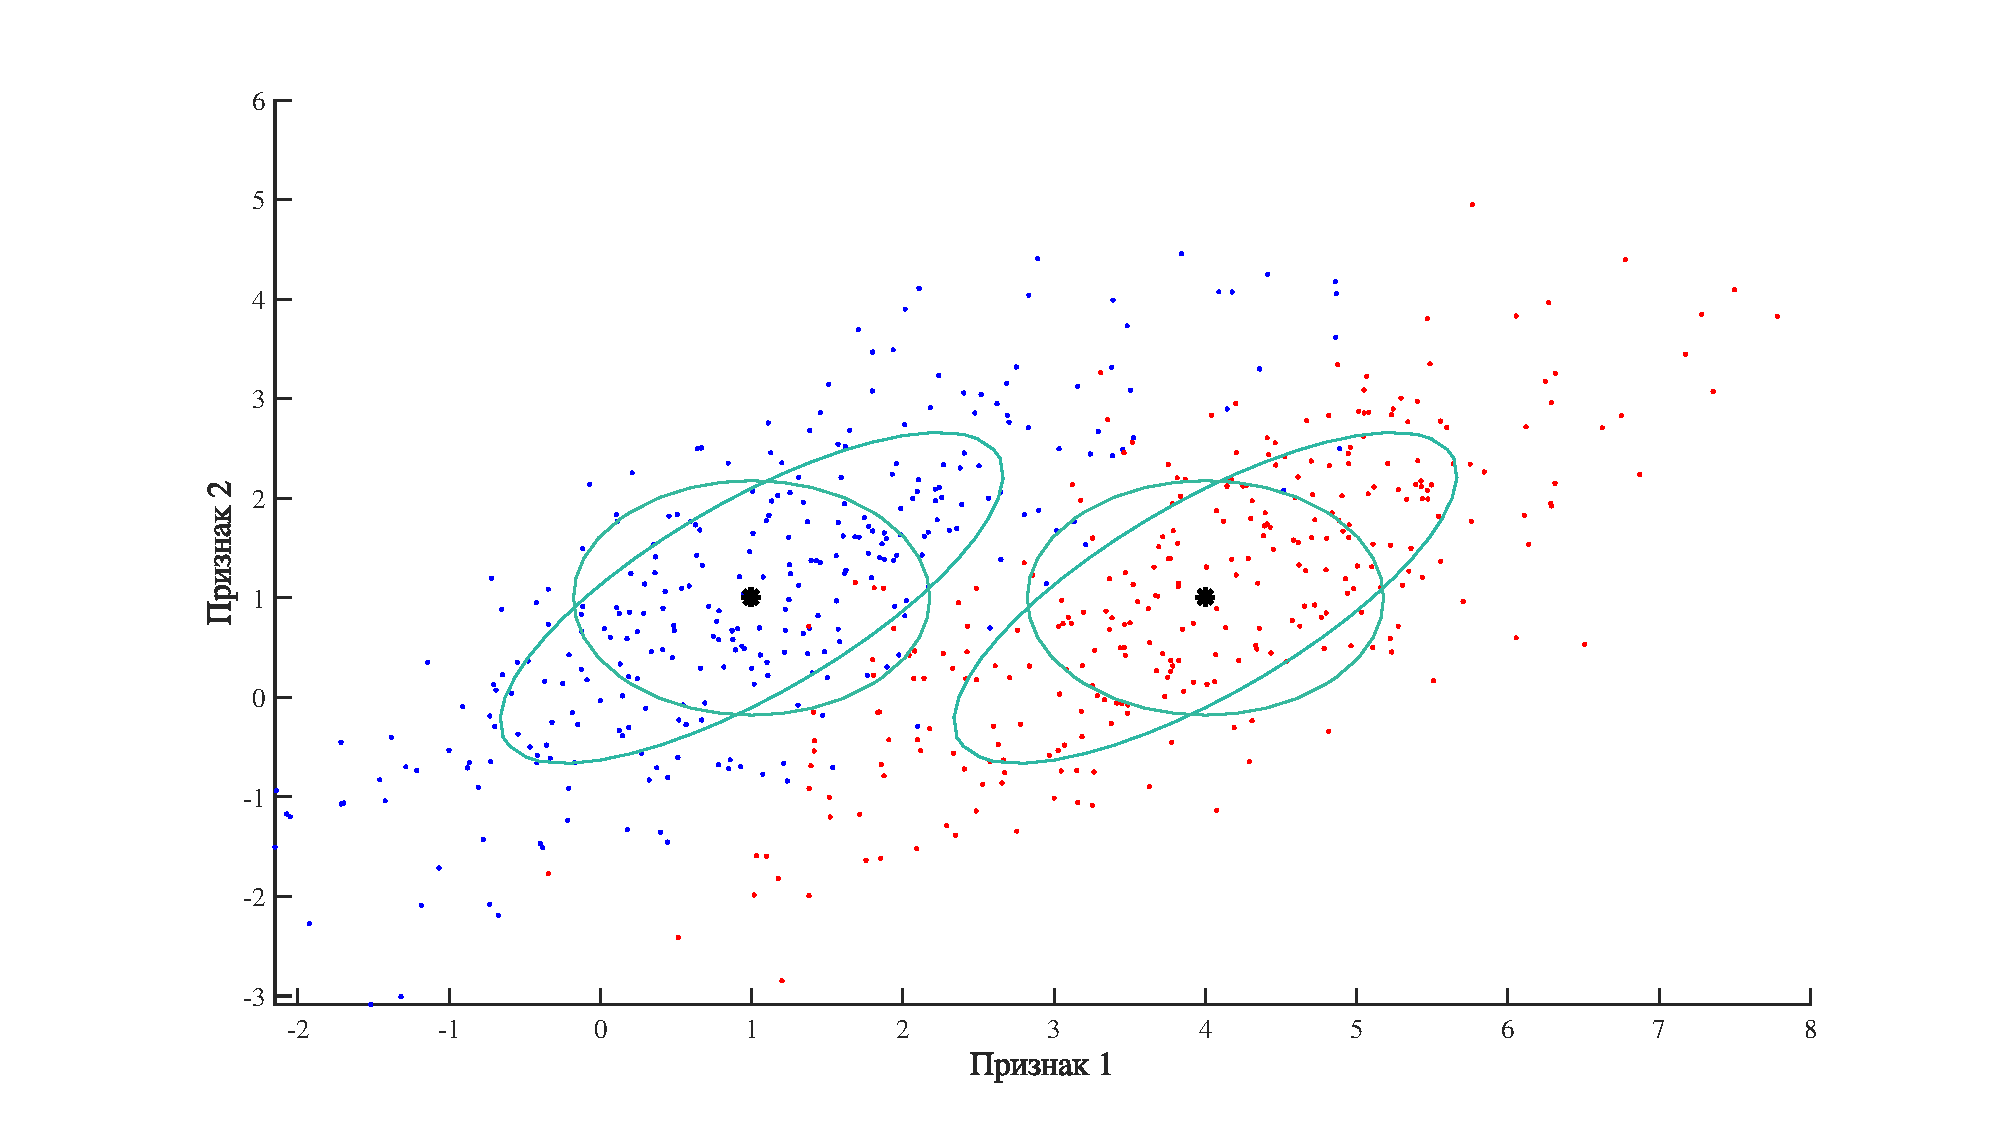
\includegraphics[width=1\linewidth]{fig/true_distribution}}
    \caption{Истинное распределение двумерных модельных данных}
\end{figure}






На рисунках заметно улучшение результатов кластеризации.
Измеренная точность кластеризации алгоритма $k$-средних составила 0,76,
алгоритма адаптивного метрического обучения~--- 0,94, что говорит о работоспособности данного подхода.
\begin{figure} %[!ht]
    \center{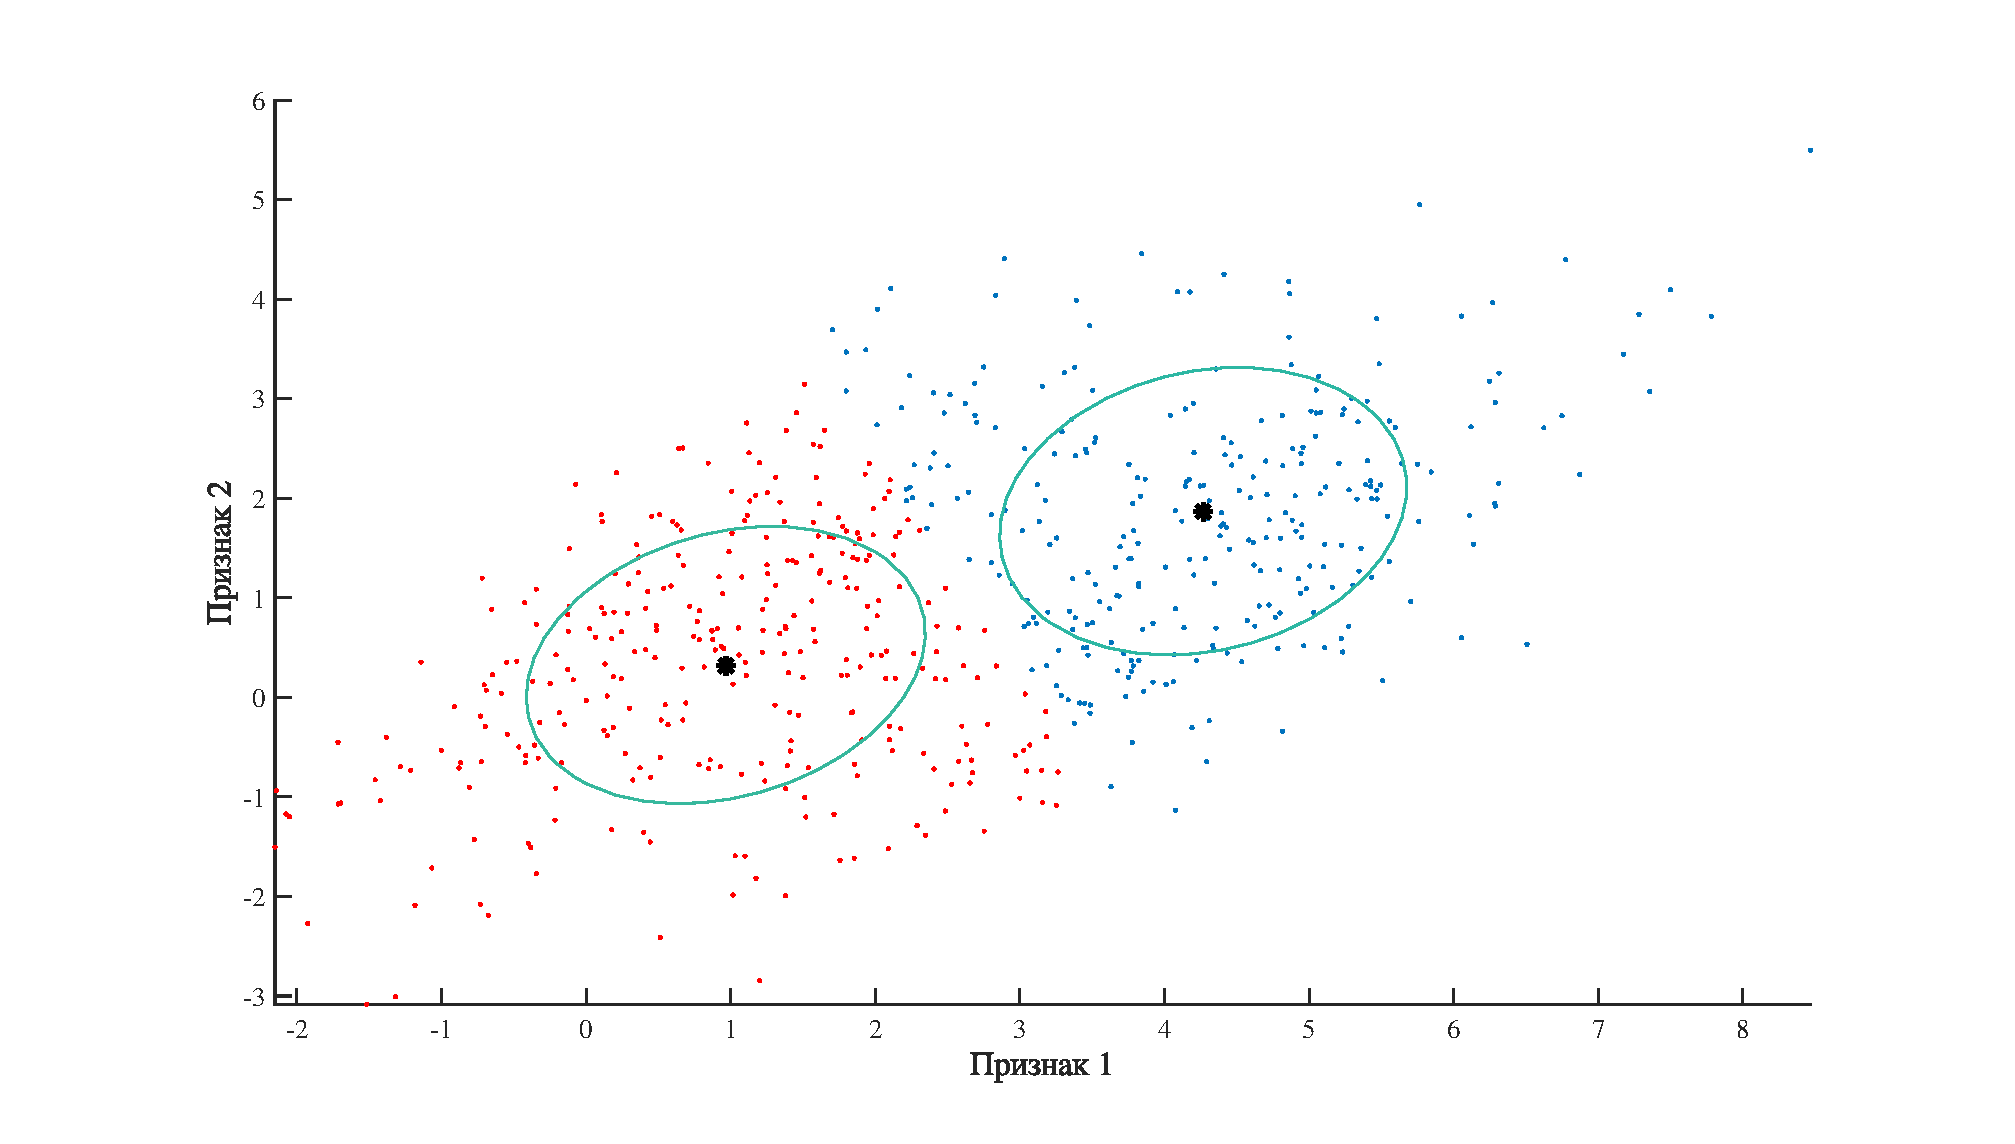
\includegraphics[width=1\linewidth]{fig/kmeans_clustering}}
    \caption{Результат кластеризации алгоритмом $k$-средних}
\end{figure}
\begin{figure} %[!ht]
    \center{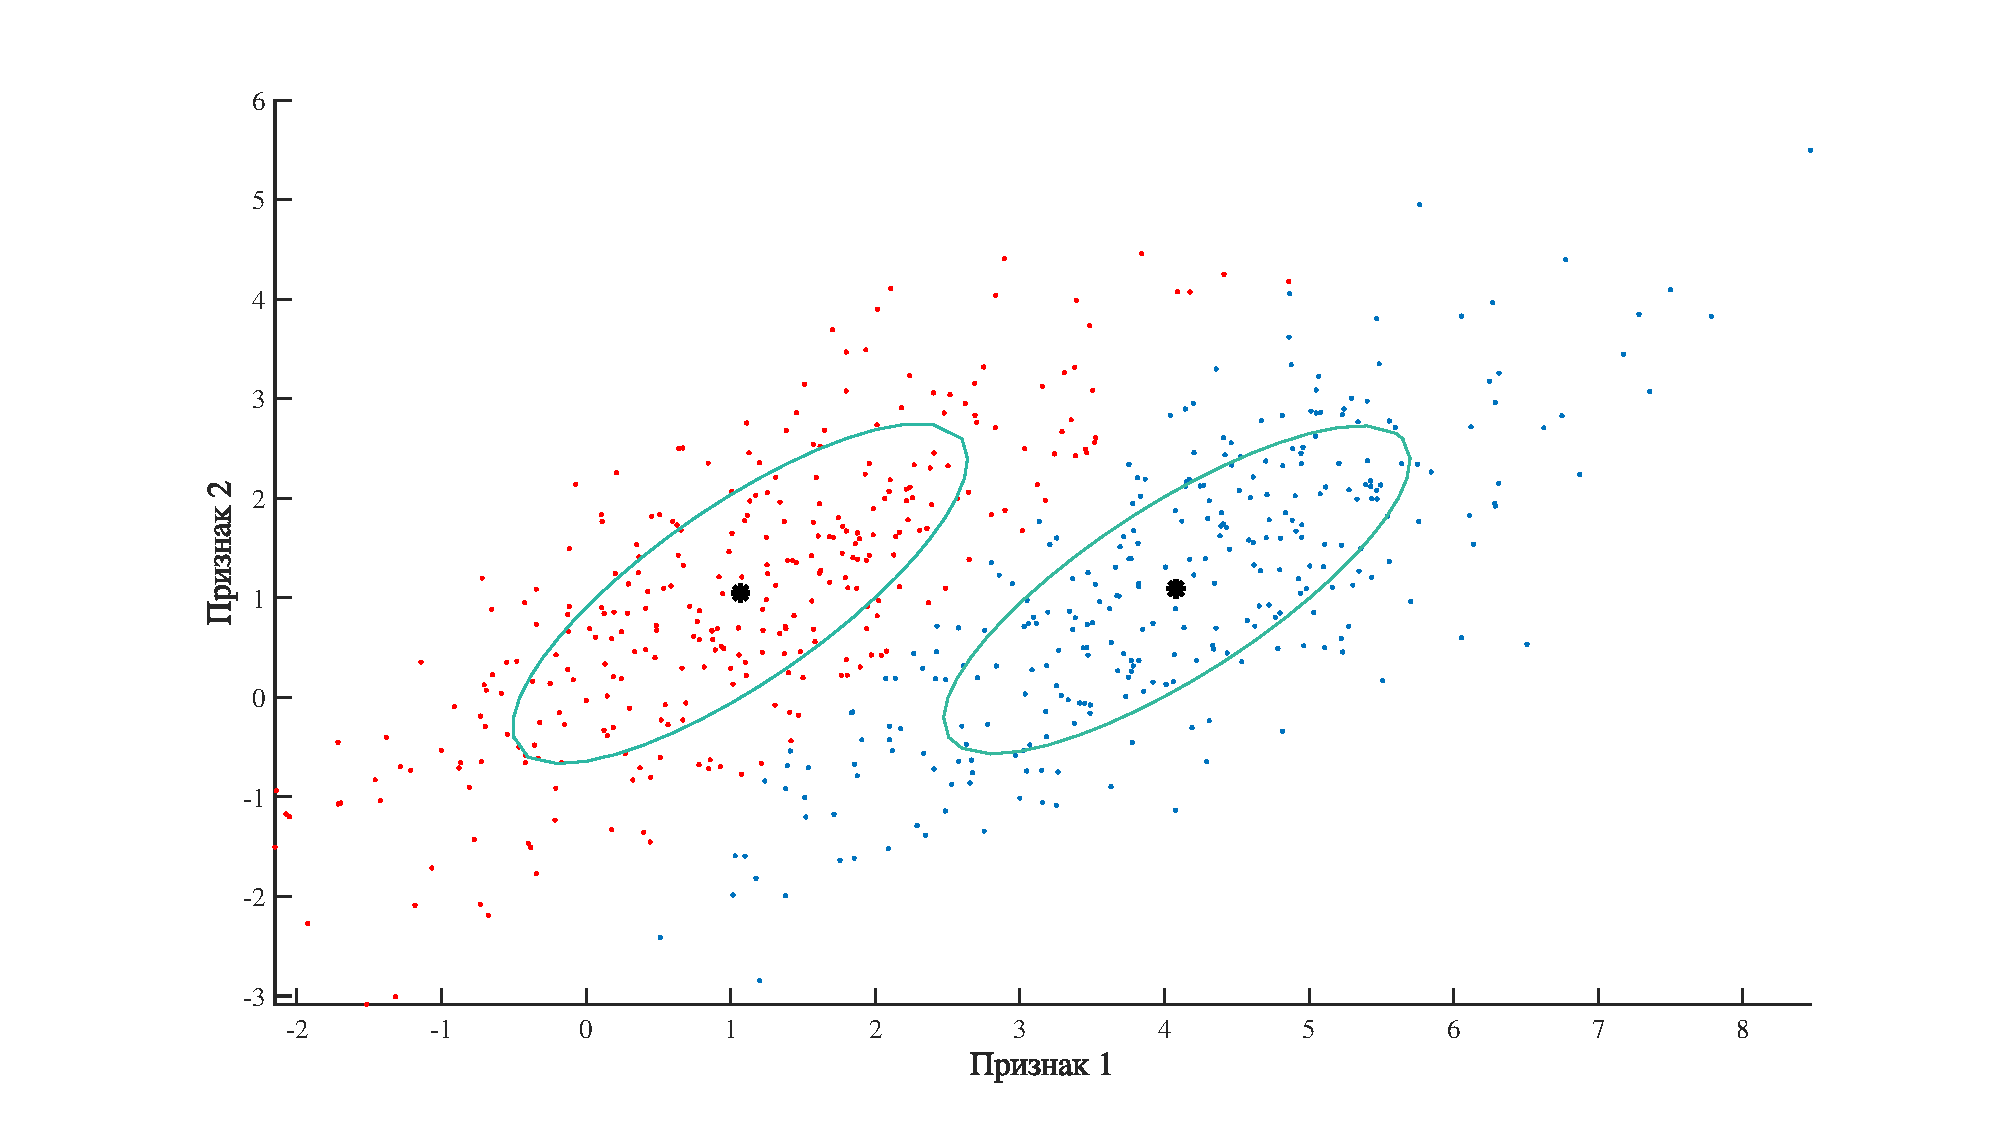
\includegraphics[width=1\linewidth]{fig/AML_clustering}}
    \caption{Результат кластеризации алгоритмом адаптивного метрического обучения}
\end{figure}


Таблица~$1$ показывает результаты вычислительного эксперимента на реальных
данных.
Алгоритм был применен к $5$ выборкам, взятых из репозитория UCI~\cite{letterrecognition, opt_digits, seeds, image, breast}.
Оценкой качества кластеризации служит число правильно кластеризованных объектов.
При клас\-те\-ри\-за\-ции объектов на более чем два класса возникает проблема соотнесения истинных классов с полученными кластерами.
Данная проблема была формализована в виде задачи о назначениях и решена с помощью венгерского алгоритма. Вычислительный эксперимент на реальных данных показал увеличение точности кластеризации при использовании метрического обучения.
\begin{table} %[!ht]
\centering
\caption{Результаты кластеризации}
\label{my-label}

\vspace{2ex}

\begin{tabular}{|l|l|l|}
\hline
\multicolumn{1}{|c}{Выборка}                  & \multicolumn{2}{c|}{Качество кластеризации} \\ \cline{2-3}
                                          & $k$-средних               & AML                 \\
\hline
Letter Recognition                        & 0,356                 & \textbf{0,428}             \\
Optical Recognition of Handwritten Digits & 0,758                 & \textbf{0,790}               \\
Seeds                                     & 0,833                 & \textbf{0,881}            \\
Image Segmentation                        & 0,545                 & \textbf{0,737}            \\
Breast Cancer Wisconsin                   & \textbf{0,960}                 & 0,956               \\ \hline
\end{tabular}
\end{table}

\section{Заключение}
В данной работе предложен новый способ снижения размерности задачи кластеризации объектов на заданное число кластеров.
Сравнивались результаты кластеризации базового алгоритма $k$-средних и алгоритма адаптивного метрического обучения. Проведен вычислительный эксперимент на синтетических данных.
Он показал наглядную интерпретацию алгоритма адаптивного метрического обучения и улучшение качества кластеризации. Вычислительный эксперимент на реальных данных показал эффективность данного подхода в реальных задачах.

Авторы выражают благодарность В. В. Стрижову за постановку задачи и внимательное отношение к работе.
%\newpage

\bigskip
%\bibliographystyle{jmlda_rus}
%\bibliography{lib}
\renewcommand{\bibname}{Литература}
\begin{thebibliography}{10}
\def\selectlanguageifdefined#1{
\expandafter\ifx\csname date#1\endcsname\relax
\else\selectlanguage{#1}\fi}

\bibitem{yang2006distance} %1
\selectlanguageifdefined{english}
\BibAuthor{Yang~L., Jin~R.}
Distance metric learning: A comprehensive survey.
          Michigan State University, 2006.  Vol.~2. 51~p.

\bibitem{bellet2013survey} %2
\selectlanguageifdefined{english}
\BibAuthor{Bellet~A., Habrard~A., Sebban~M.}
A survey on metric learning for feature vectors and structured data.
ArXiv:1306.6709,   2013.

\bibitem{guillaumin2009you} %3
\selectlanguageifdefined{english}
\BibAuthor{Guillaumin~M., Verbeek~J., Schmid~C.}
Is that you? Metric learning approaches for face identification~//
IEEE 12th  Conference (International) on Computer Vision Proceedings, 2009.
 P.~498--505.

\bibitem{yang2006efficient}
\selectlanguageifdefined{english}
\BibAuthor{Yang~L., Jin~R., Sukthankar~R., Liu~Y.}
An efficient algorithm for local distance metric learning~//
AAAI, 2006. Vol.~2. P.~543--548.

\bibitem{globerson2005metric} %5
\selectlanguageifdefined{english}
\BibAuthor{Globerson~A., Roweis~S.~T.}
Metric learning by collapsing classes~//
Advances in neural information processing systems~/
Eds.\ Y.~Weiss, B.~Sch\"{o}lkopf, J.~Platt.~--- Cambridge, MA, USA: MIT Press,
2005. Vol.~18. P.~451--458.

\bibitem{xing2003distance} %6
\selectlanguageifdefined{english}
\BibAuthor{Xing~E.\,P., Ng~A.\,Y., Jordan~M.\,I., Russell~S.}
Distance metric learning with application to clustering with
  side-information~//
Advances in Neural Information Processing Systems,
2003. Vol.~15. P.~505--512.

\bibitem{geurts2001pattern} %7
\selectlanguageifdefined{english}
\BibAuthor{Geurts~P.}
Pattern extraction for time series classification~//
Principles of data mining and knowledge discovery.~---
Springer, 2001. P.~115--127.

\bibitem{friedl1997decision} %8
\selectlanguageifdefined{english}
\BibAuthor{Friedl~M.~A., Brodley~C.~E.}
Decision tree classification of land cover from remotely sensed data~//
Remote Sensing of Environment, 1997. Vol.~61. No.\,3. P.~399--409.

\bibitem{hyafil1976constructing} %9
\selectlanguageifdefined{english}
\BibAuthor{Hyafil~L., Rivest~R.\,L.}
Constructing optimal binary decision trees is np-complete~//
Inform. Proc. Lett., 1976. Vol.~5. No.\,1. P.~15--17.

\bibitem{dy2004feature} %10
\selectlanguageifdefined{english}
\BibAuthor{Dy~J.\,G., Brodley~C.\,E.}
Feature selection for unsupervised learning~//
J.~Machine Learning Res., 2004. Vol.~5. P.~845--889.

\bibitem{ye2007adaptive} %11
\selectlanguageifdefined{english}
\BibAuthor{Ye~J., Zhao~Z., Liu~H.}
Adaptive distance metric learning for clustering~//
IEEE Conference on Computer Vision and Pattern Recognition, 2007.
P.~1--7.

\bibitem{macqueen1967some} %12
\selectlanguageifdefined{english}
\BibAuthor{MacQueen~J., et~al.}
Some methods for classification and analysis of multivariate observations~//
5th Berkeley Symposium on Mathematical Statistics and
Probability Proceedings, 1967. Vol.~1. P.~281--297.

\bibitem{ding2005equivalence} %13
\selectlanguageifdefined{english}
\BibAuthor{Ding~C., He~X., Simon~H.~D.}
On the equivalence of nonnegative matrix factorization and spectral
clustering~//
SIAM Data Mining Conference Proceedings, 2005.  P.~606--610.

\bibitem{shawe2004kernel} %14
\selectlanguageifdefined{english}
\BibAuthor{Shawe-Taylor~J., Cristianini~N.}
Kernel methods for pattern analysis.~--- Cambridge University Press,
2004. 478~p.

\bibitem{letterrecognition} %15
\selectlanguageifdefined{english}
Letter recognition dataset.
\url{http://archive.ics.uci.edu/ml/machine-learning-databases/letter-recognition/}.

\bibitem{opt_digits}
\selectlanguageifdefined{english}
Optical recognition of handwritten digits dataset.
\url{http://archive.ics.uci.edu/ml/machine-learning-databases/optdigits/}.

\bibitem{seeds}
\selectlanguageifdefined{english}
Seeds dataset.
\url{http://archive.ics.uci.edu/ml/machine-learning-databases/00236/}.

\bibitem{image}
\selectlanguageifdefined{english}
Image segmentation dataset dataset.
\url{http://archive.ics.uci.edu/ml/machine-learning-databases/image/}.

\bibitem{breast}
\selectlanguageifdefined{english}
Breast cancer wisconsin dataset.
  \url{http://archive.ics.uci.edu/ml/machine-learning-databases/breast-cancer-wisconsin/}.
\Russian
\end{thebibliography}

\maketitleSecondary
\English
%\bibliographystyle{jmlda_eng}
%
\renewcommand{\bibname}{References}
\begin{thebibliography}{10}
\def\selectlanguageifdefined#1{
\expandafter\ifx\csname date#1\endcsname\relax
\else\selectlanguage{#1}\fi}

\bibitem{yang2006distance}
\selectlanguageifdefined{english}
Yang, L.,  and R.~Jin.
2006. Distance metric learning: A~comprehensive survey.
{Michigan State University}. Vol.~2. 51~p.

\bibitem{bellet2013survey}
\selectlanguageifdefined{english}
Bellet, A., A.~Habrard,  and M.~Sebban.
2013.
A survey on metric learning for feature vectors and structured data.
{arXiv:1306.6709}.

\bibitem{guillaumin2009you}
\selectlanguageifdefined{english}
Guillaumin, M., J.~Verbeek,  and C.~Schmid.
2009. Is that you? Metric learning approaches for face identification.
\BibJournal{IEEE 12th Conference (International) on Computer Vision Proceedings}.
498--505.

\bibitem{yang2006efficient}
\selectlanguageifdefined{english}
Yang, L., R.~Jin, R.~Sukthankar,  and Y.~Liu.
2006. An efficient algorithm for local distance metric learning.
\BibJournal{AAAI} 2:543--548.

\bibitem{globerson2005metric}
\selectlanguageifdefined{english}
Globerson, A.,  and S.\,T. Roweis.
2005. Metric learning by collapsing classes.
\BibTitle{Advances in neural information processing systems}.
Eds.\ Y.~Weiss, B.~Sch\"{o}lkopf, and J.~Platt.
Cambridge, MA, USA: MIT Press. 18:451--458.

\bibitem{xing2003distance}
\selectlanguageifdefined{english}
Xing, E.\,P., A.\,Y. Ng, M.\,I. Jordan,  and S.~Russell.
2003. Distance metric learning with application to clustering with side-information.
\BibJournal{Advances in Neural Information Processing Systems}
15:505--512.

\bibitem{geurts2001pattern}
\selectlanguageifdefined{english}
Geurts, P.
2001. Pattern extraction for time series classification.
\BibTitle{Principles of data mining and knowledge discovery}.
Springer. 115--127.

\bibitem{friedl1997decision}
\selectlanguageifdefined{english}
Friedl, M.\,A.,  and C.\,E.~Brodley.
1997. Decision tree classification of land cover from remotely sensed data.
\BibJournal{Remote Sensing of Environment}
61(3):399--409.

\bibitem{hyafil1976constructing}
\selectlanguageifdefined{english}
Hyafil, L.,  and R.\,L. Rivest.
1976. Constructing optimal binary decision trees is np-complete.
\BibJournal{Inform. Proc. Lett.} 5(1):15--17.

\bibitem{dy2004feature}
\selectlanguageifdefined{english}
Dy, J.\,G.,  and C.\,E. Brodley.
2004. Feature selection for unsupervised learning.
\BibJournal{J.~Machine Learning Res.} 5:845--889.

\bibitem{ye2007adaptive}
\selectlanguageifdefined{english}
Ye, J., Z.~Zhao,  and H.~Liu.
2007. Adaptive distance metric learning for clustering.
\BibJournal{IEEE Conference
  on Computer Vision and Pattern Recognition}. 1--7.

\bibitem{macqueen1967some}
\selectlanguageifdefined{english}
MacQueen, J., \textit{et~al}.
1967. Some methods for classification and analysis of multivariate observations.
\BibJournal{5th Berkeley Symposium on Mathematical Statistics
  and Probability Proceedings}. 1(14):281--297.

\bibitem{ding2005equivalence}
\selectlanguageifdefined{english}
Ding, C., X.~He,  and H.\,D. Simon.
2005. On the equivalence of nonnegative matrix factorization and spectral clustering.
\BibJournal{SIAM Data Mining Conference Proceedings}. 606--610.

\bibitem{shawe2004kernel}
\selectlanguageifdefined{english}
Shawe-Taylor, J.,  and N.~Cristianini.
2004.
\BibTitle{Kernel methods for pattern analysis}.
Cambridge University Press. 478~p.

\bibitem{letterrecognition}
\selectlanguageifdefined{english}
Letter recognition dataset.
Available at:
  \url{http://archive.ics.uci.edu/ml/machine-learning-databases/letter-recognition/}
(accessed March~28, 2016).

\bibitem{opt_digits}
\selectlanguageifdefined{english}
Optical recognition of handwritten digits dataset.
Available at:
  \url{http://archive.ics.uci.edu/ml/machine-learning-databases/optdigits/}
(accessed March~28, 2016).

\bibitem{seeds}
\selectlanguageifdefined{english}
Seeds dataset.
Available at:
  \url{http://archive.ics.uci.edu/ml/machine-learning-databases/00236/}
(accessed March~28, 2016).

\bibitem{image}
\selectlanguageifdefined{english}
Image segmentation dataset dataset.
Available at:
  \url{http://archive.ics.uci.edu/ml/machine-learning-databases/image/}
(accessed March~28, 2016).

\bibitem{breast}
\selectlanguageifdefined{english}
Breast cancer wisconsin dataset.
Available at:
  \url{http://archive.ics.uci.edu/ml/machine-learning-databases/breast-cancer-wisconsin/}
(accessed March~28, 2016).

\end{thebibliography}

\end{document}

